\documentclass[xcolor=svgnames]{beamer}
\mode<presentation>
{
      \setbeamertemplate{footline}[page number]
      \setbeamercovered{transparent}
      \setbeamertemplate{navigation symbols}{}
      \usecolortheme[named=DarkGreen]{structure}
}

\usepackage[english]{babel}
\usepackage{times}
\usepackage{CJKutf8}
\usepackage{graphics}

\begin{document}
\begin{CJK*}{UTF8}{gbsn}


\title{操作系统服务、结构及系统调用}

\author{李中国}
\institute{苏州大学计算机科学与技术学院}
%\date{2011年5月30日}
\date{}

\begin{frame}
  \titlepage
\end{frame}


\begin{frame}{操作系统提供的服务}
%\begin{itemize}
%\item 用户界面 --- 图形界面(GUI), 命令行界面(CLI)
%\item 执行用户程序 
%\item I/O操作
%\item 文件系统操作(文件与目录的创建、删除、读写、搜索、权限管理...)
%\item 
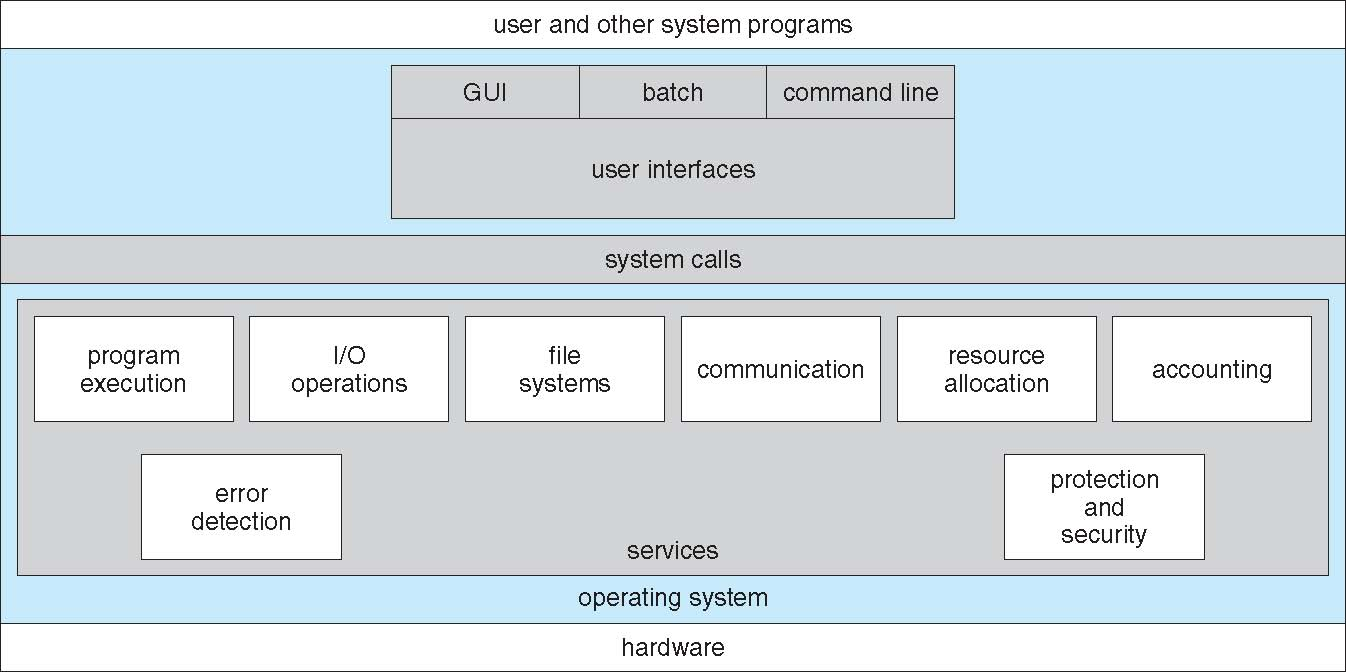
\includegraphics[width=1.0\textwidth]{services.jpg}
%\end{itemize}
\end{frame}

\begin{frame}{用户界面:命令行界面}
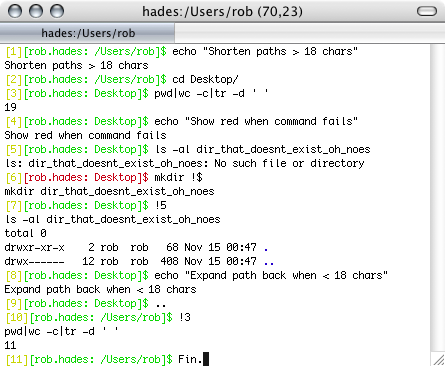
\includegraphics[width=1.0\textwidth]{bash.png}
\end{frame}

\begin{frame}{用户界面:图形用户界面}
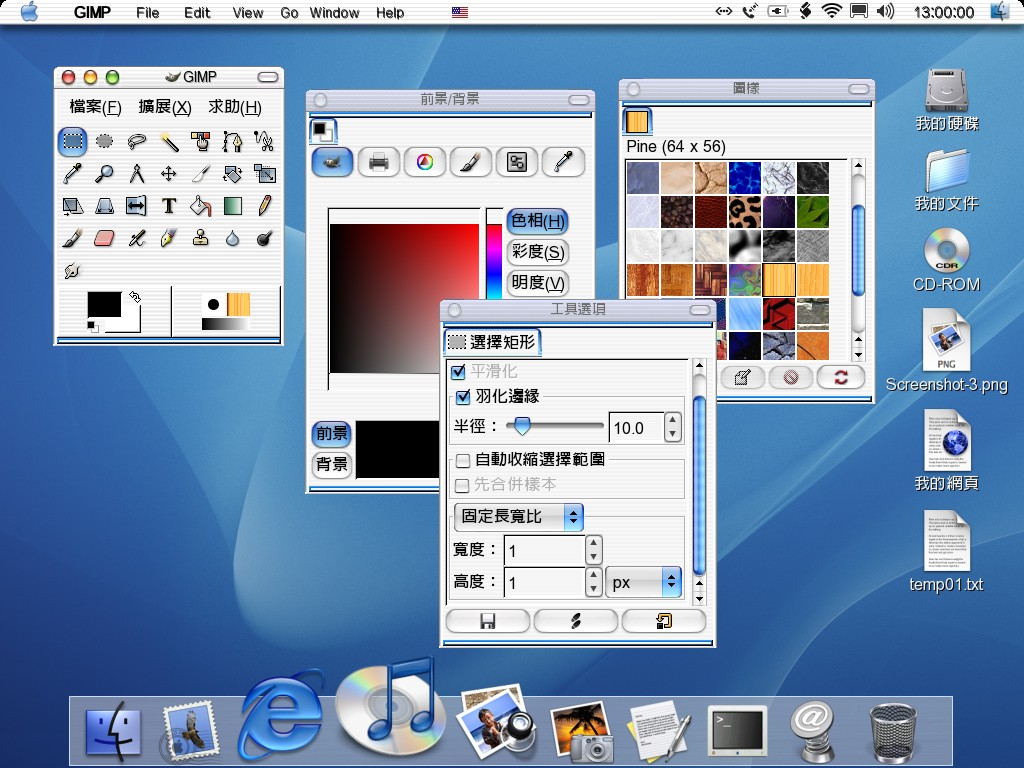
\includegraphics[width=1.0\textwidth]{macos.jpg}
\end{frame}

\begin{frame}{思考及演示:CLI与GUI的优缺点对比}
\begin{itemize}
\item Demo 1 --- word frequency counting
\item Demo 2 --- lines of C source code 
\end{itemize}
\end{frame}

\begin{frame}{系统调用}
\begin{itemize}
\item CLI/GUI是人使用操作系统时的界面
\item 系统调用可看作获取操作系统服务的编程界面(接口)
\item 一般可用C/C++编写
\item 通常将系统调用封装成API方便使用
\item 常见API:
\begin{itemize}
\item Win32 API
\item POSIX API (Unix, Linux, Mac OS X)
\item Java API
\end{itemize}
\end{itemize}
\end{frame}

\begin{frame}{系统调用示例: 文件拷贝}
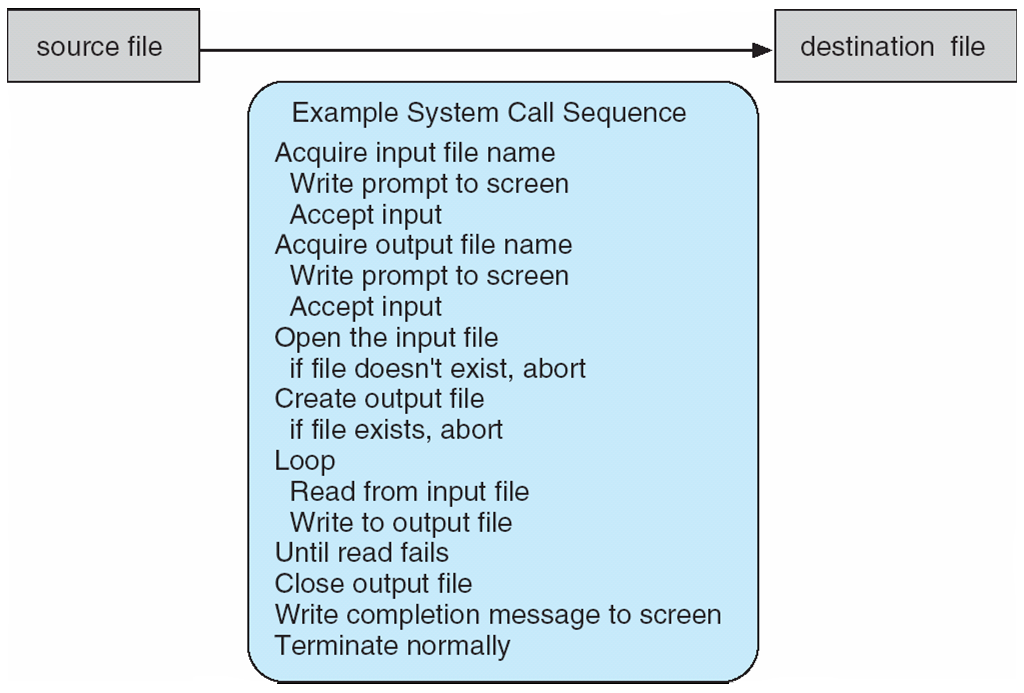
\includegraphics[width=1.0\textwidth]{syscall.png}
\end{frame}

\begin{frame}{API -- 系统调用 -- 操作系统之间的关系}
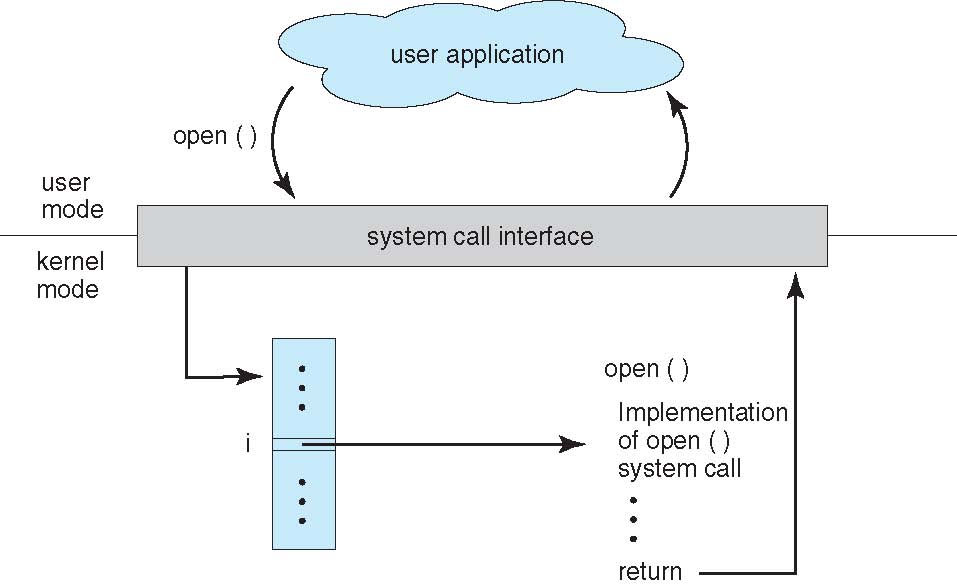
\includegraphics[width=1.0\textwidth]{syscall-os.jpg}
\end{frame}

\begin{frame}{API -- 系统调用 -- 操作系统之间的关系: 标准C函数库的例子}
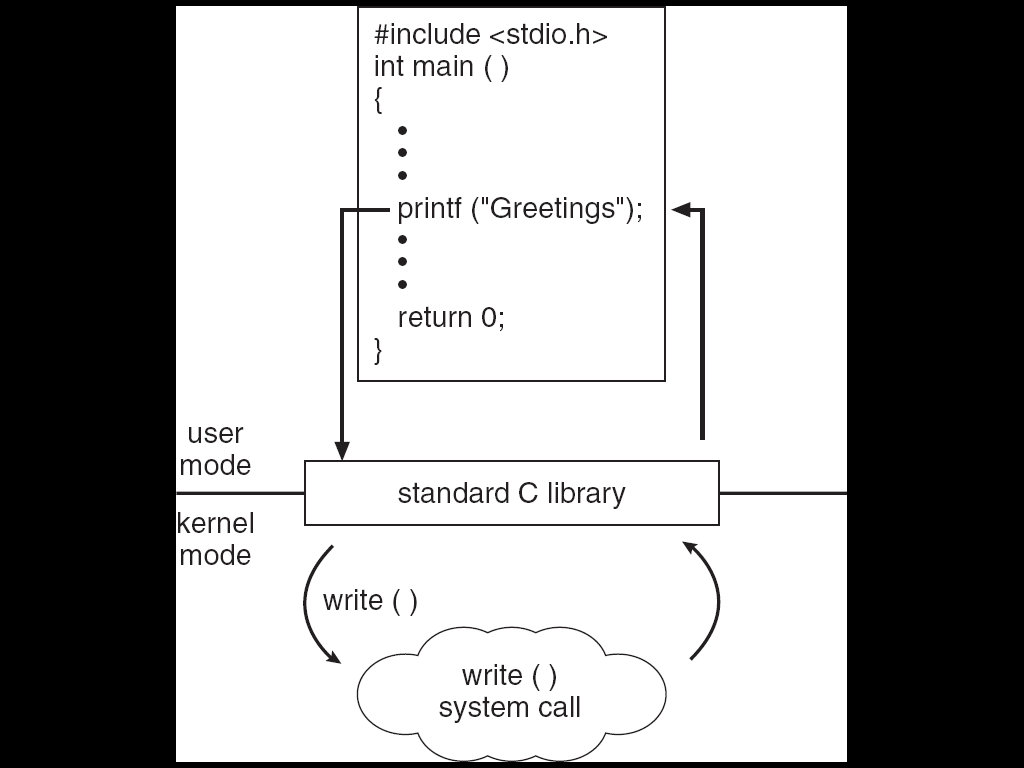
\includegraphics[width=1.0\textwidth]{printf.png}
\end{frame}

\begin{frame}{系统调用的例子}
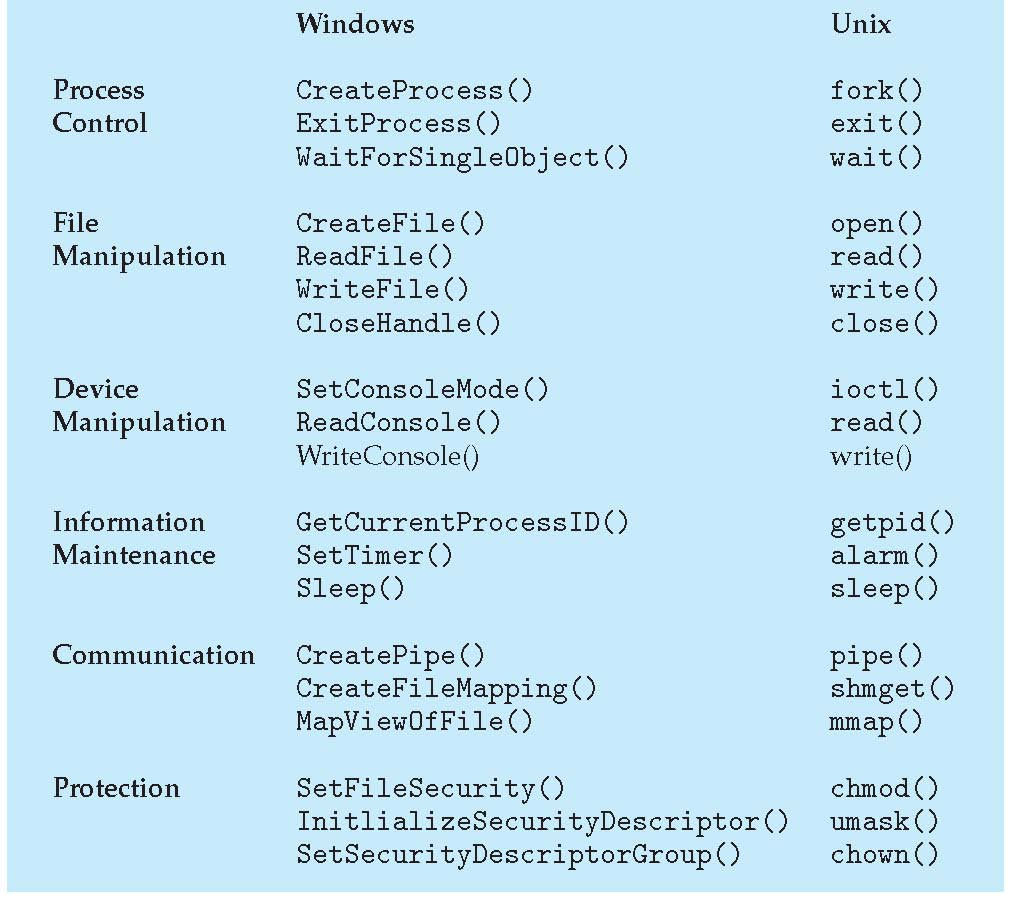
\includegraphics[width=0.9\textwidth]{examples.jpg}
\end{frame}

\begin{frame}{系统程序(system programs)}
%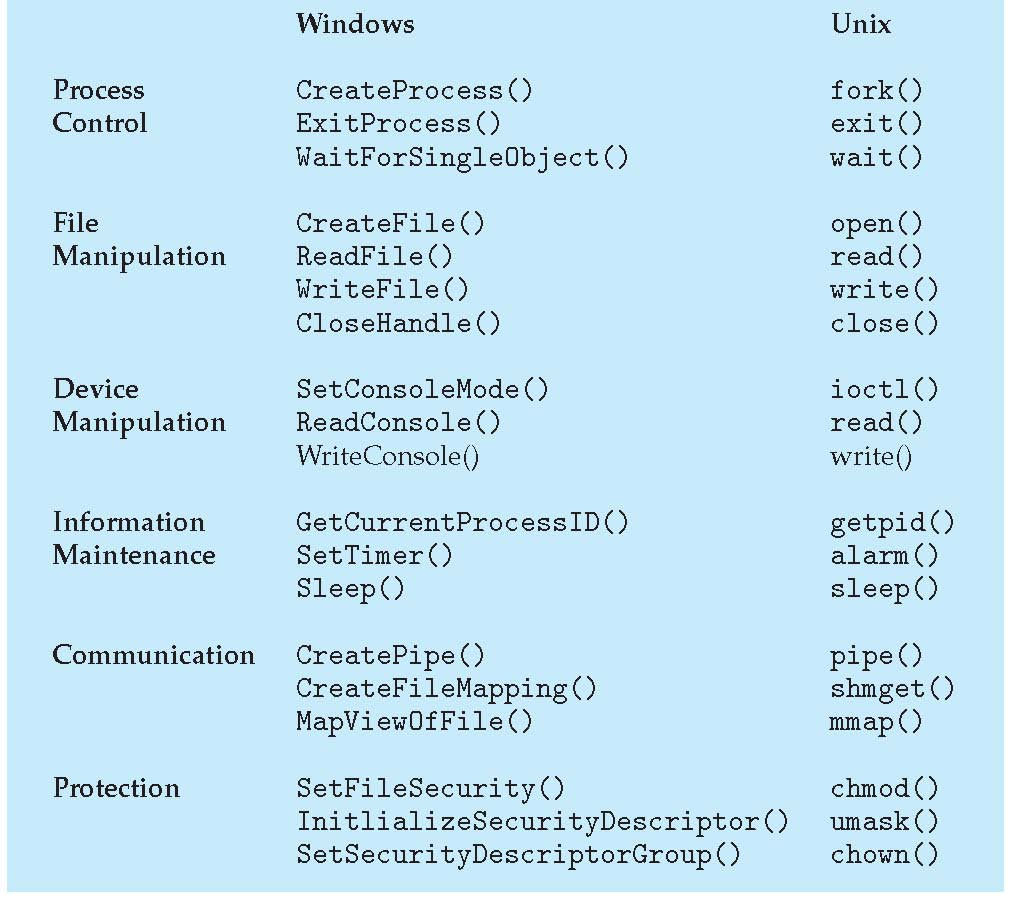
\includegraphics[width=0.9\textwidth]{examples.jpg}
\begin{itemize}
\item 操作系统提供的用于系统管理等任务的程序
\item 某些系统程序只是系统调用的接口程序(例如删除文件)
\item 文件管理程序
\begin{itemize}
\item touch
\item rm
\item cp
\item rename
\item mkdir
\end{itemize}
\item 编程语言相关的程序
\begin{itemize}
\item 编译器
\item 汇编器
\item 调试器
\item 解释器
\end{itemize}
\end{itemize}
\end{frame}

\end{CJK*}
\end{document}
